\setcounter{section}{2}
This section describes search results obtained using a TF-IDF ranked retrieval.

\subsection{Ranked Retrieval}
For one word, documents are given in descending order according to their TF-IDF score.

\begin{equation}
tf\_idf_{d,t} = \frac{tf_{d,t}}{len_d} * idf_t
\end{equation}

\begin{equation}
idf_t = log_{10}(\frac{N}{df_t})
\end{equation}

Using $log(1+tf_{dt})$ instead of $tf_{d,t}$ should decrease the impact of the term frequency, giving more importance to the document length.

To the contrary, using $\sqrt{len_d}$ instead of $len_d$ will give more importance to the number of occurences and less to the document length.

\textbf{zombie}\\
\begin{verbatim}
Found 36 matching document(s)

 0. .\davisWiki\JasonRifkind.f   0,28571
 1. .\davisWiki\Zombie_Walk.f   0,04403
 2. .\davisWiki\EmilyMaas.f   0,01923
 3. .\davisWiki\AliciaEdelman.f   0,01852
 4. .\davisWiki\Kearney_Hall.f   0,01786
 5. .\davisWiki\Spirit_Halloween.f   0,01639
 6. .\davisWiki\Zombies_Reclaim_the_Streets.f   0,01471
 7. .\davisWiki\StevenWong.f   0,01266
 8. .\davisWiki\Measure_Z.f   0,01190
 9. .\davisWiki\Scream.f   0,01105
\end{verbatim}

\textbf{attack}\\
\begin{verbatim}
Found 228 matching document(s)

 0. .\davisWiki\Measure_Z.f   0,02381
 1. .\davisWiki\TheWarrior.f   0,02326
 2. .\davisWiki\Kearney_Hall.f   0,01786
 3. .\davisWiki\Muilop.f   0,01493
 4. .\davisWiki\bg-33p.f   0,01370
 5. .\davisWiki\Furly707.f   0,01299
 6. .\davisWiki\s.martin.f   0,01205
 7. .\davisWiki\TrustInMe.f   0,01136
 8. .\davisWiki\Thong_H._Huynh.f   0,01053
 9. .\davisWiki\PamAarkes.f   0,01042
\end{verbatim}

\subsection{Ranked Multiword Retrieval}
The following scores are obtained by computing the cosine similarity between the query vector (containing the value 1 for each token in the query, doubles are removed) and the vector of each document containing the TF-IDF score of each token in the query for the given document.

To reduce the computation time, each vector is first normalized before computing any similarities:

\begin{equation}
\vec{d} = \frac{\vec{d}}{\|\vec{d}\|_{L2}} = \frac{\vec{d}}{\sqrt{\sum{d_i^2}}}
\end{equation}

Each similarity is then computed using 

\begin{equation}
cos(\vec{q}, \vec{d}) = \vec{q} \cdot \vec{d} = \sum{q_i d_i}
\end{equation}

\textbf{zombie attack}\\
\begin{verbatim}
Found 249 matching document(s)

 0. .\davisWiki\JasonRifkind.f   1,03751
 1. .\davisWiki\Zombie_Walk.f   0,16877
 2. .\davisWiki\Kearney_Hall.f   0,11537
 3. .\davisWiki\Measure_Z.f   0,11060
 4. .\davisWiki\Spirit_Halloween.f   0,08272
 5. .\davisWiki\EmilyMaas.f   0,06983
 6. .\davisWiki\AliciaEdelman.f   0,06725
 7. .\davisWiki\TheWarrior.f   0,06581
 8. .\davisWiki\Scream.f   0,05576
 9. .\davisWiki\Zombies_Reclaim_the_Streets.f   0,05340
\end{verbatim}

\textbf{money transfer}\\
\begin{verbatim}
Found 1602 matching document(s)

 0. .\davisWiki\MattLM.f   0,42137
 1. .\davisWiki\Angelique_Tarazi.f   0,28830
 2. .\davisWiki\JordanJohnson.f   0,26085
 3. .\davisWiki\Transfer_Student_Services.f   0,19108
 4. .\davisWiki\NicoleBush.f   0,11908
 5. .\davisWiki\Title_Companies.f   0,10534
 6. .\davisWiki\Munch_Money.f   0,09775
 7. .\davisWiki\money.f   0,09631
 8. .\davisWiki\Anthony_Swofford.f   0,09130
 9. .\davisWiki\Transfer_Student_Association.f   0,08931
\end{verbatim}

\textbf{sleeping on campus}\\
\begin{verbatim}
Found 9886 matching document(s)

 0. .\davisWiki\Campus_Pay_Phones.f   0,58616
 1. .\davisWiki\Campus_Safety.f   0,43962
 2. .\davisWiki\CJB.f   0,43962
 3. .\davisWiki\Campus_Unions.f   0,37682
 4. .\davisWiki\100_Dollar_Coupon_Book.f   0,35169
 5. .\davisWiki\CEVS.f   0,35169
 6. .\davisWiki\F.U.C.K..f   0,35169
 7. .\davisWiki\FUCK.f   0,35169
 8. .\davisWiki\JoshHorne.f   0,30098
 9. .\davisWiki\Pinon_Apartments.f   0,30098
\end{verbatim}

\textbf{Why do we use a union query here, but an intersection query in Assignment 1?}

Since the first assignment did not have any ranking measure and sorting, an intersection query was required to return only relevant results (since the first result was as relevant as any other).

Now, thanks to the cosine similarity and TF-IDF score, we are able to sort the results by relevance. Therefore, we can take a larger dataset since the ranking shall guarantee that the first result is relevant, and will usually contain every term of the query.


\subsection{What is a good search result?}
\subsubsection{Relevance estimation issues}
\begin{itemize}
    \item skiing trip $\Rightarrow$ 441 documents
    \begin{itemize}
        \item \url{https://daviswiki.org/Capital\_Ski\_\%26\_Sports\_Club} $\Rightarrow$  1 or 2? (2, lots of ski references, but no trip)
        \item \url{https://daviswiki.org/Transit\_Destinations} $\Rightarrow$  0 or 1? (0, lots of mention to trip, but not to ski)
        \item \url{https://daviswiki.org/DeannaBeals} $\Rightarrow$  0 or 0? (1, user profile but lots of mention to ski)
    \end{itemize}
    \item university rowing team $\Rightarrow$ 2417 documents
    \begin{itemize}
        \item \url{https://daviswiki.org/University\_House\_Annex} $\Rightarrow$  0 or 1? (1, not mention of the team but university facility)
        \item \url{https://daviswiki.org/UC_Davis_Judo_Club} $\Rightarrow$  0 or 1? (1, not about rowing but about university teams)
        \item \url{https://daviswiki.org/Sacramento_State_University} $\Rightarrow$  0 or 1? (1, about university teams)
    \end{itemize}
    \item tourist attractions $\Rightarrow$ 41 documents
    \begin{itemize}
        \item \url{https://daviswiki.org/Dixon} $\Rightarrow$  2 or 3? (2, tourist attractions, but very few references)
        \item \url{https://daviswiki.org/Central\_Coast} $\Rightarrow$  2 or 3? (3, wide document but gives hints)
        \item \url{https://daviswiki.org/San_Francisco} $\Rightarrow$  0 or 1? (1, nor about Davis or tourists, but gives a few links to attractions)
    \end{itemize}
    
\subsubsection{Precision and recall}
Using the following formulas, we calculate the precision and recall for each query:
\begin{equation}
precision = \frac{|\{relevant\_documents\}\cap\{retrieved\_documents\}|}{|\{retrieved\_documents\}|}
\end{equation}

Precision describes the relevance of the retrieved documents, i.e. the amount of junk retrieved. It is the number of correct results divided by the number of results returned by the query.

\begin{equation}
recall = \frac{|\{relevant\_documents\}\cap\{retrieved\_documents\}|}{|\{relevant\_documents\}|}
\end{equation}

Recall gives an information about the completeness of our search engine, i.e. how many relevant documents have been retrieved divided by the number of relevant documents.\\

skiing trip:
\begin{itemize}
\item $precision_{10} = \frac{6}{10}$, $recall_{10} = \frac{6}{1000}$
\item $precision_{20} = \frac{9}{20}$, $recall_{20} = \frac{9}{1000}$
\end{itemize}

university rowing team
\begin{itemize}
\item $precision_{10} = \frac{4}{10}$, $recall_{10} = \frac{4}{1000}$
\item $precision_{20} = \frac{8}{20}$, $recall_{20} = \frac{8}{1000}$
\end{itemize}

tourist attractions
\begin{itemize}
\item $precision_{10} = \frac{9}{10}$, $recall_{10} = \frac{9}{1000}$
\item $precision_{20} = \frac{13}{20}$, $recall_{20} = \frac{13}{1000}$
\end{itemize}

\begin{figure}[H]
\centering
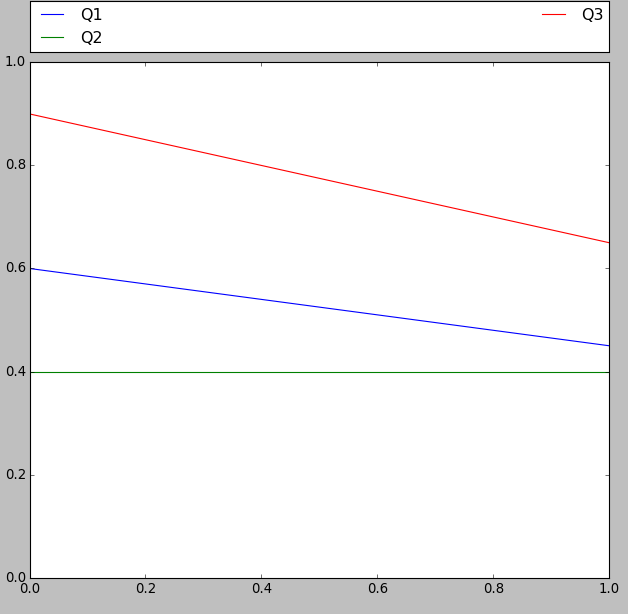
\includegraphics[width=0.6\linewidth]{img/precision.png}
\caption{Precision considering the first 10 and 20 results for each request}
\end{figure}

\begin{figure}[H]
\centering
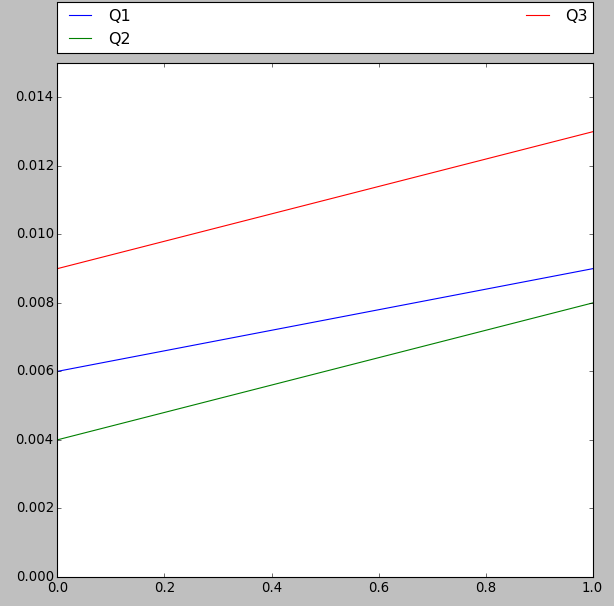
\includegraphics[width=0.6\linewidth]{img/recall.png}
\caption{Recall considering the first 10 and 20 results for each request}
\end{figure}


\textit{Which precision is the highest? Is it different for different queries? Are there any trends?}

We can observe that the precision is usually higher when taking into account only the 10 first results than for the 20 first results. This means that our ranking is relevant, and that we have less interesting results when looking at document with a lower similarity score.
\\

\textit{Which recall is the highest? Is it different for different queries? Are there any correlation between precision at 10, precision at 20, recall at 10, and recall at 20 for the same query?}

Obviously, the more results we consider, the higher the recall. This fact can be observed for every query.
\\

\textit{Does ranked retrieval in general give a higher or lower precision, higher or lower recall than unranked retrieval? Why is that?}

Considering the 10 or 20 best best results for the ranked retrieval will always result in a lower precision than an intersection query. This is due to the fact that only a few documents contain every term in the query, so most documents are not so relevant.

However, for any number of documents, the recall will always be higher for the ranked retrieval since it returns far more document than the intersection query and try to return first the most relevant documents.


\subsection{Computing PageRank with Power Iteration}
Our implementation of the power iteration algorithm uses a sparse transition matrix according to the following formulas:

If a link from \textit{i} to \textit{j} exists the probability to move from \textit{i} to \textit{j} is  $P(i,j) = c * \frac{1}{N} + P_{jump}$

With $c = 0.85$ the probability to move from \textit{i} to \textit{j} using an existing link. Therefore, $1 - c$ is the probability to move from \textit{i} to any document.

\textit{N} is the number of documents.

$P_{jump}$ is the probability to arrive on the current document by jumping from another one. $P_{jump} = (1 - c) * \frac{1}{N}$

Eventually, the probability to move from \textit{i} to \textit{j} if there is no link between them is $P_{jump}$ if \textit{i} has at least one output link, $\frac{1}{N}$ otherwise.

We obtain the following 50 highest results after 6 iterations (epsilon = 0.0001):
\begin{verbatim}
RANKING: DOC_NAME SCORE
1: 121 0,008040
2: 21 0,007848
3: 245 0,007353
4: 1531 0,005120
5: 1367 0,002862
6: 31 0,002517
7: 80 0,002192
8: 1040 0,002146
9: 254 0,002024
10: 452 0,001931
11: 157 0,001653
12: 169 0,001628
13: 392 0,001592
14: 100 0,001576
15: 3870 0,001474
16: 561 0,001451
17: 997 0,001332
18: 202 0,001268
19: 8 0,001258
20: 884 0,001240
21: 72 0,001221
22: 145 0,001208
23: 27 0,001085
24: 645 0,001076
25: 2883 0,001075
26: 490 0,001069
27: 81 0,001033
28: 942 0,001006
29: 125 0,000968
30: 247 0,000941
31: 337 0,000885
32: 708 0,000879
33: 179 0,000871
34: 1403 0,000867
35: 152 0,000861
36: 484 0,000838
37: 26 0,000836
38: 321 0,000830
39: 242 0,000811
40: 1964 0,000785
41: 1043 0,000778
42: 857 0,000755
43: 1755 0,000748
44: 1200 0,000723
45: 281 0,000713
46: 154 0,000713
47: 16 0,000706
48: 1153 0,000704
49: 1365 0,000703
50: 3692 0,000694
\end{verbatim}

The first document is https://daviswiki.org/davis, while the $50^{th}$ is https://daviswiki.org/interpreting\%20user\%20statistics. This seems a reasonable ranking since many pages link to Davis, and far less to Interpreting User Statistics. Most of the pages linking to the first document may also have a higher ranking than the $50^{th}$ document, resulting in a higher score for Davis.

In average, we can observe that the lower the ranking, the less are the links pointing towards the document.


\subsection{Monte-Carlo PageRank Approximation}
\begin{figure}[H]
\centering
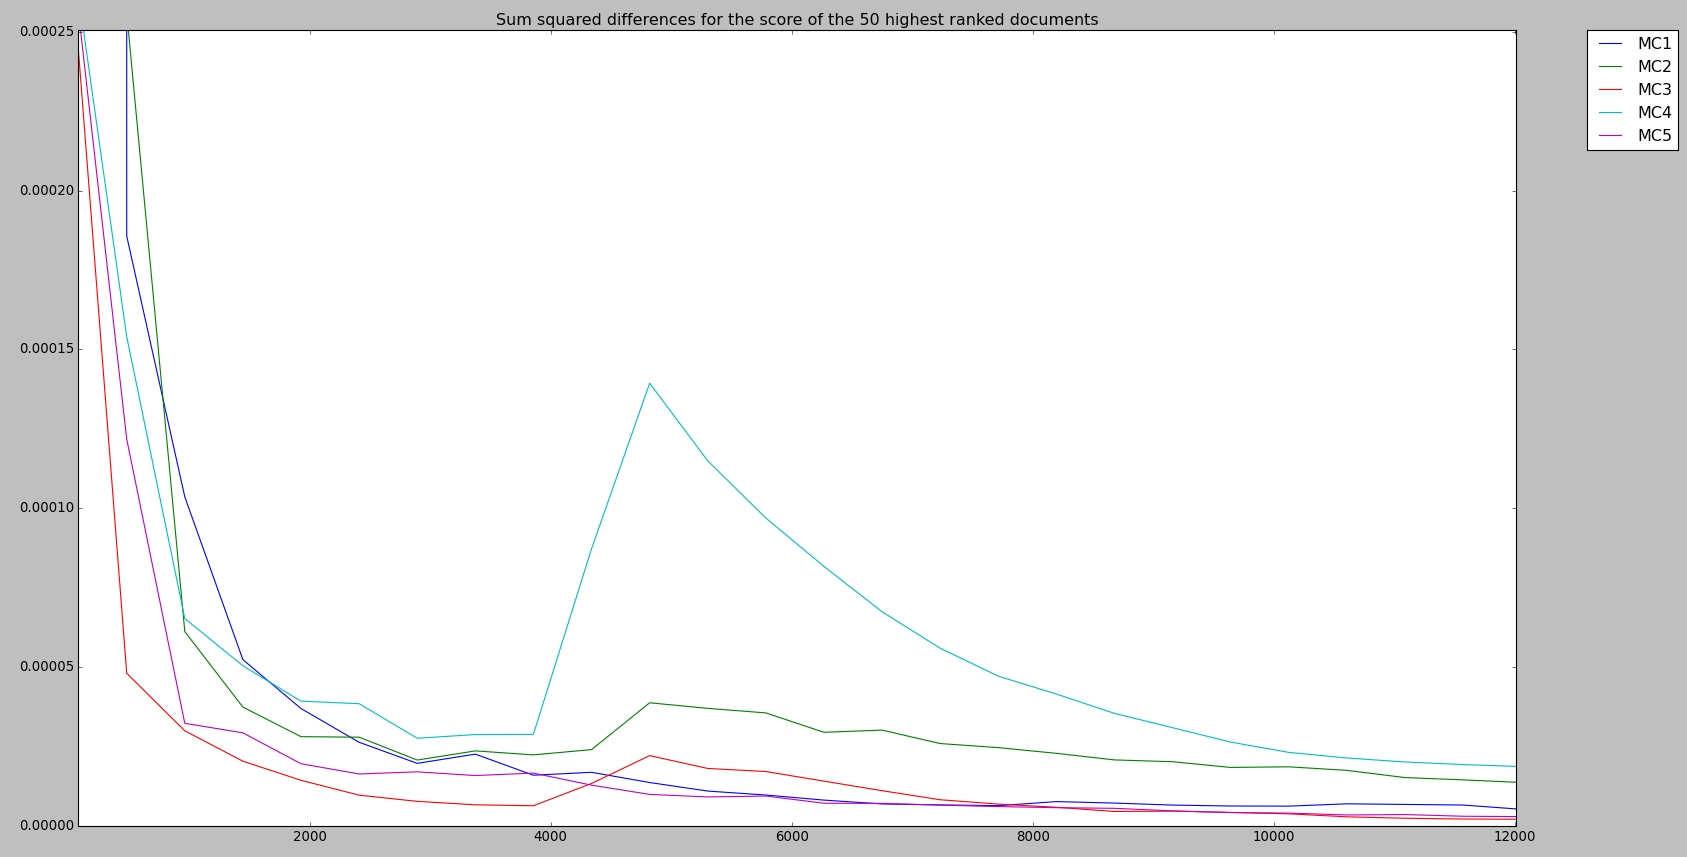
\includegraphics[width=0.8\linewidth]{img/high.png}
\caption{Sum Squared Error of the 50 highest ranked documents}
\end{figure}

\begin{figure}[H]
\centering
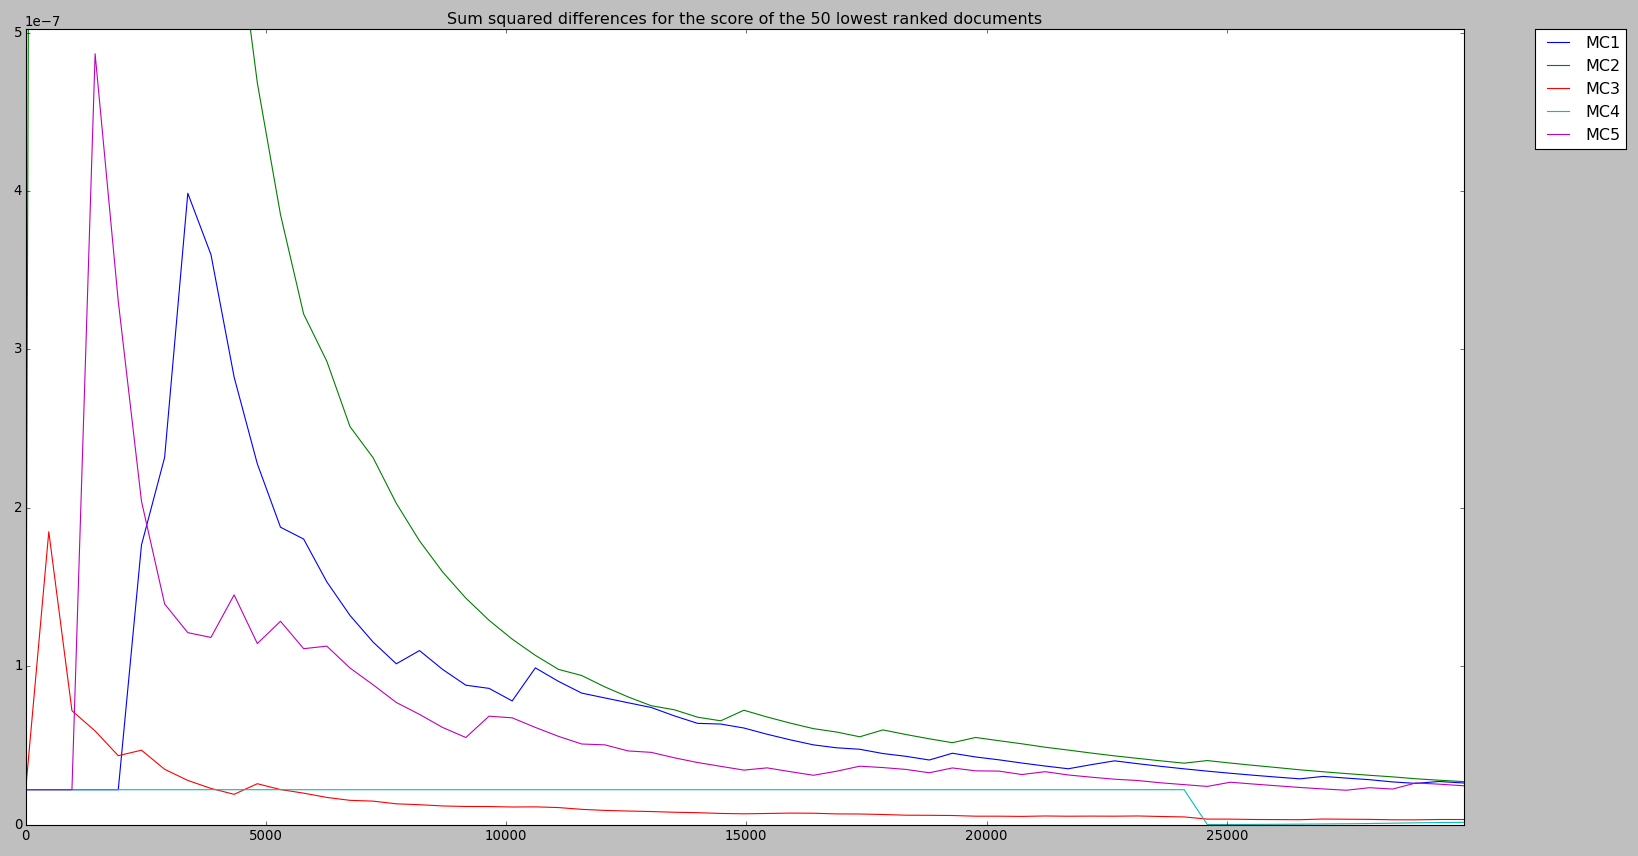
\includegraphics[width=0.8\linewidth]{img/low.png}
\caption{Caption}
\end{figure}


\textit{Do your findings about the difference between the five method variants and the dependence of N support the claims made in the paper by Avrachenkov et al.?}\\

The paper stated that one iteration of MC5 was enough to have a good estimate of the most important pages. This is not confirmed by our curves, showing a really slow convergence for MC1, 2 and 5.\\

Indeed, our best algorithm is here MC4 (complete path starting m times at each node) while MC5 is far slower to converge.\\

Therefore, we can observe that, and in agreement with the paper, the two end-point methods have the worst performances. We can also see that cyclic methods have better performances than random start ones.\\

Eventually, we see that high ranked documents converge far faster that low ranked documents.\\

\textit{What do you see? Why do you get this result? Explain and relate to the properties of the (probabilistic) Monte-Carlo methods in contrast to the (deterministic) power iteration method.}\\
We observe very unexpected results for MC3 (MC complete path with cycling start), which look like hyperbols. Those may be caused by cycles in our graph. However, similar results should also be observed for MC4 since the only difference between MC3 and 4 is that 4  stops when reaching a dangling node.

\subsection{Combine tf-idf and PageRank}

\textit{What is the effect of letting the tf-idf score dominate this ranking? What is the effect of letting the pagerank dominate? What would be a good strategy for selecting an "optimal" combination? (Remember the quality measures you studied in Task 2.3.)}\\

If TF-IDF dominates, the ranking of a page will depend the document content, how does this content matches the query terms, whereas a higher weight for the pagerank will give first popular results on the Web.\\

The optimal combination would be obtained by trying various weights and asking people to rate the results returned for each query. Therefore, the combination giving the best results in terms or recall or precision (depending on the user needs) will be chosen.

\end{itemize}
